\chapter{About Mininet-WiFi}

Mininet-WiFi is a fork of the Mininet SDN network emulator and extended the functionality of Mininet by adding virtualized WiFi stations and access points based on the standard Linux wireless drivers and the 80211\_hwsim wireless simulation driver. We added classes to support the addition of these wireless devices in a Mininet network scenario and to emulate the attributes of a mobile station such as position and movement relative to the access points.

The Mininet-WiFi extended the base Mininet code by adding or modifying classes and scripts. So, Mininet-WiFi adds new functionality and still supports all the normal SDN emulation capabilities of the standard Mininet network emulator.


\section{Requirements}\index{requirements}

Mininet-WiFi should work fine in any Ubuntu Distribution from 14.04.

\section{Installing Mininet-WiFi}\index{installing}

\subsection{GitHub}\index{github}
You have to follow only for 4 steps to install Mininet-WiFi:

\begin{itemize}
\item sudo apt-get install git
\item git clone https://github.com/intrig-unicamp/mininet-wifi
\item cd mininet-wifi
\item sudo util/install.sh -Wnfv\\
\end{itemize}

Mininet WiFi is installed by a script. Run the script with the \texttt{-h help} option to see all the options available.

\begin{minted}{bash}
    wifi:~$ util/install.sh -h
\end{minted}

\subsection{Docker}\index{docker}
Mininet-WiFi is available on \underline{\href{https://registry.hub.docker.com/u/ramonfontes/mininet-wifi/}{Docker}}\footnote{https://registry.hub.docker.com/u/ramonfontes/mininet-wifi/}.

\section{Limitations}\index{limitations}
Mininet-WiFi inherits all limitations of Mininet, including:
\begin{itemize}
\item You cannot handle with packets that go out to the incoming port with the OpenFlow protocol.
\end{itemize}

\section{Architecture and Components}\index{arch}

The main components that make part of the development of Mininet-WiFi are illustrated in Figure~\ref{flowchart}. In the kernel-space the module \textit{mac80211\_hwsim} is responsible for creating virtual Wi-Fi interfaces, important for stations and access points. Continuing in the kernel-space, MLME (\textit{Media Access Control Sublayer Management Entity})\footnote{some of the functions performed by MLME are authentication, association, sending and receiving \textit{beacons}, etc.}  is realized in the stations side, while in the user-space the \textit{hostapd} is responsible  for this task in the AP side.

Mininet-WiFi also uses a couple utilities such as \textit{iw}, \textit{iwconfig} e o \textit{wpa\_supplicant}. The first two are used for interface configuration and for getting information from wireless interfaces and the last one is used with \textit{Hostapd}, in order to support WPA (\textit{Wi-Fi Protected Access}), among other things. Besides them, another fundamental utility is \textit{TC} (\textit{Traffic Control}). The \textit{TC} is an user-space utility program used to configure the Linux kernel packet scheduler, responsible for controlling the rate, delay, latency and loss, applying these attributes in virtual interfaces of stations and APs, representing with higher fidelity the behavior of the real world.


\begin{figure}[!t]
  \centering
{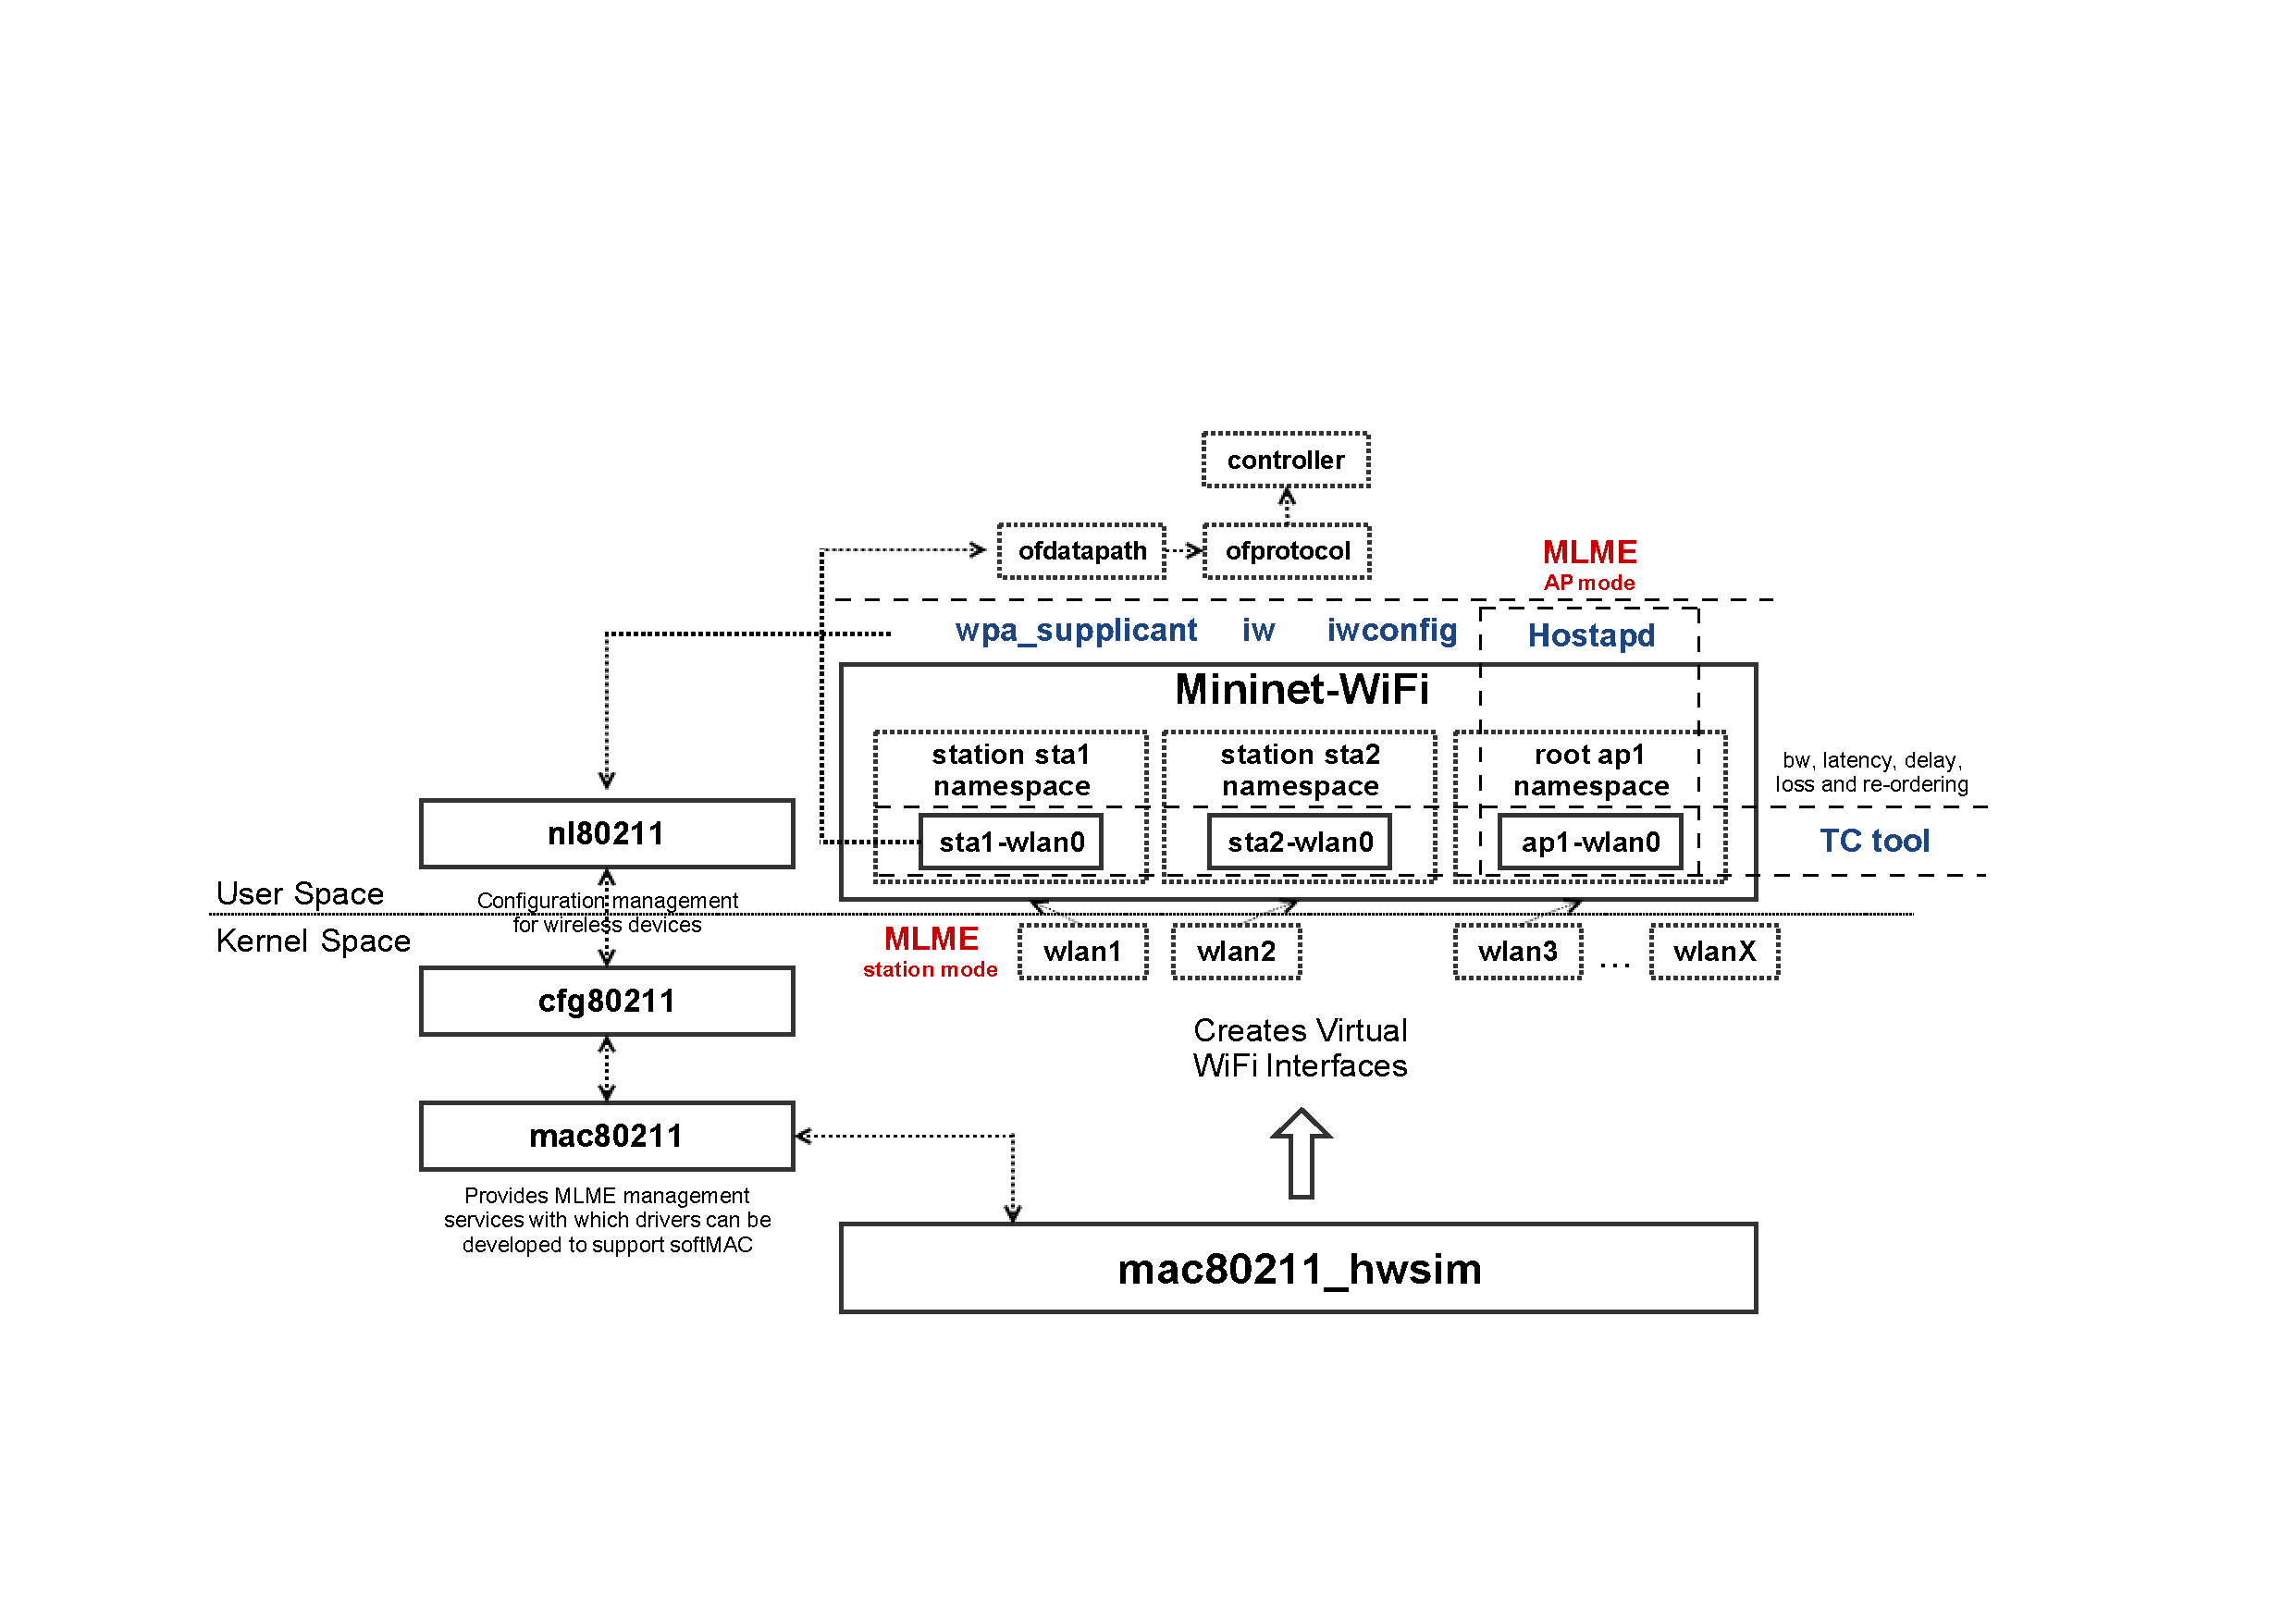
\includegraphics[trim=3.7cm 5cm 2.1cm 7.8cm,clip,width=1.1\textwidth]{Pictures/components}}
  \caption{Mininet-WiFi Components.}
   \label{flowchart}
\end{figure}

\begin{figure}[!t]
\centering
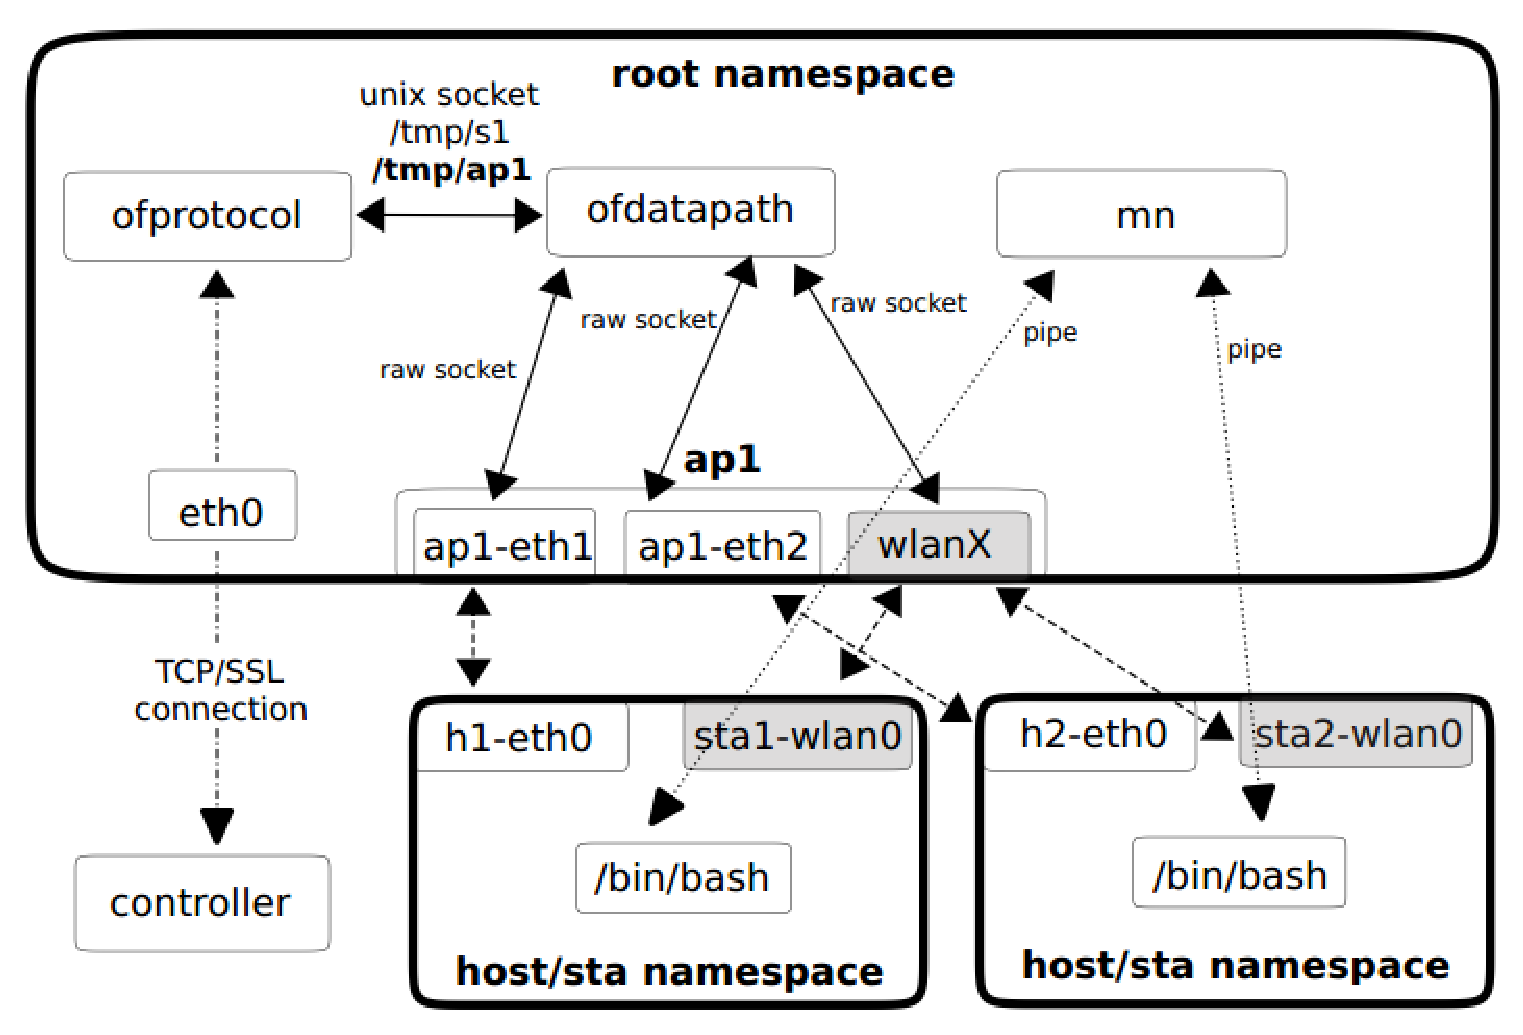
\includegraphics[width=0.7\textwidth]{Pictures/arch.eps}
\caption{Components and connections in a two-host network created with Mininet-WiFi.}
\label{fig:arch}
\end{figure}

Figure~\ref{fig:arch} depicts the components and connections in a simple topology with two stations (or hosts) created with Mininet-WiFi, where the newly implemented components (highlighted in gray) are presented along the original Mininet building blocks. Although stations are equipped with a wireless interface by default they are able to connect with access points through wired links (veth pairs) as well.  

More specifically, we added WiFi interfaces on stations that now are able to connect to an access point through its (\texttt{wlanX}) interface that is bridged to an OpenFlow switch with AP capabilities represented by (\texttt{ap1}). 
Similar to Mininet, the virtual network is created by placing host processes in Linux OS network namespaces interconnected through virtual Ethernet (veth) pairs. The wireless interfaces to virtualize WiFi devices work on \textit{master} mode for access points and \textit{managed} mode for stations.

\noindent \textbf{Stations:} Are devices that connect to an access point through authentication and association. In our implementation, each station has one wireless card (\texttt{staX-wlan0} - where X shall be replaced by the number of each station). Since the traditional Mininet hosts are connected to an access point, stations are able to communicate with those hosts.

\noindent \textbf{Access Points:} Are devices that manage associated stations. Virtualized through \texttt{hostapd}\footnote{Hostapd (\textbf{H}ost \textbf{A}ccess \textbf{P}oint \textbf{D}aemon) user space software capable of turning normal wireless network interface cards into access points and authentication servers} daemon and use virtual wireless interfaces for access point and authentication servers. 
While virtualized access points do not have (yet) APIs allowing users to configure several parameters in the same fashion of a real one, the current implementation covers the most important features, for example ssid, channel, mode, password, cryptography, etc.

Both stations and access points use \texttt{cfg80211} to communicate with the wireless device driver, a Linux 802.11 configuration API that provides communication between stations and \texttt{mac80211}. This framework in turn communicates directly with the WiFi device driver through a \texttt{netlink} socket (or more specifically \texttt{nl80211}) that is used to configure the \texttt{cfg80211} device and for kernel-user-space communication as well.

\subsection{Files}

\begin{itemize}
\item mininet/wifiAdHocConnectivity.py - checking adhoc pairs
\item mininet/wifiAssociationControl.py - association Control techniques
\item mininet/wifiLink.py - link details
\item mininet/wifiDevices.py - specification of real devices
\item mininet/wifiMeshRouting.py - wireless mesh routing
\item mininet/wifiMobility.py - mobility parameters
\item mininet/wifiModule.py - module 
\item mininet/wifiPlot.py - graphs
\item mininet/wifiPropagationModels.py - propagation models
\item mininet/wifiReplaying.py - replaying captured traces
\item mininet/vanet.py - VANET networks
\end{itemize}

\subsection{Classes}\index{classes}

\begin{itemize}
\item \textit{UserAP():} User-space AP
\item \textit{OVSAP():} Open vSwitch AP
\item \textit{addHost():} adds a host to a topology and returns the host name
\item \textit{addAccessPoint():} adds an access point to a topology and returns the access point name
\item \textit{addCar():} adds a car to a topology and returns the car name
\item \textit{addPhysicalBaseStation():} attach a physical usb interface to a virtual base station to a topology and returns the physical base station name
\item \textit{addStation():} adds a station to a topology and returns the station name
\item \textit{addSwitch():} adds a switch to a topology and returns the switch name
\item \textit{addWirelessMeshAP():} adds an ap with wireless interface working as wireless mesh to a topology and returns the switch name
\item \textit{addLink():} adds a bidirectional link to a topology (and returns a link key, but this is not important). Links in Mininet-WiFi are bidirectional unless noted otherwise.

\item \textit{plotGraph():} use this class if you want to plot graph.
\item \textit{startMobility:} useful when you want to use a mobility model.
\end{itemize}

\section{Wireless medium emulation}

Mininet-WiFi relies on two approaches for simulating the wireless medium: tc and wmediumd.

\subsection{Traffic Control (TC)}

Tc (traffic control) is the user-space utility program used to configure the Linux kernel packet scheduler. Used to configure Traffic Control in the Linux kernel, Traffic Control consists of the following:

\begin{itemize}
  \item \textbf{Shaping:} When traffic is shaped, its rate of transmission is under control. Shaping may be more than lowering the available bandwidth - it is also used to smooth out bursts in traffic for better network behaviour. Shaping occurs on egress.
  \item \textbf{Scheduling:} By  scheduling  the  transmission  of  packets it is possible to improve interactivity for traffic  that  needs  it  while  still guaranteeing  bandwidth  to  bulk  transfers. Reordering is also called prioritizing, and happens only on egress.
  \item \textbf{Policing:} Where shaping deals with transmission of traffic, policing  pertains to traffic arriving. Policing thus occurs on ingress.
  \item \textbf{Dropping:} Traffic exceeding a set bandwidth may also be dropped forthwith, both on ingress and on egress.
\end{itemize}

The aforementioned properties have been used to apply values for bandwidth, loss, latency and delay in Mininet-WiFi. Tc was the first approach adopted in Mininet-WiFi for simulating the wireless medium.

\subsubsection{Intermediate Functional Block (IFB) Devices}\index{ifb}\label{ifb}

There are two modes of traffic shaping: \texttt{ingress} and \texttt{egress}. Ingress handles incoming traffic and egress outgoing traffic. Linux does not support shaping/queuing on ingress, but only policing. Therefore IFB exists, which we can attach to the ingress queue while we can add any normal queuing like as egress queue on the IFB device.

Intermediate Functional Block (IFB) is an alternative to tc filters for handling ingress traffic, by redirecting it to a virtual interface and treat is as egress traffic. IFB is supported by calling net.useIFB() just after adding all nodes and before calling net.configureWifiNodes(). Further information about IFB is available at \url{http://shorewall.net/traffic\_shaping.htm\#IFB}.

The main reason for ingress traffic shaping in Mininet-WiFi is that if the user want to measure the throughput between two nodes using a tool like Iperf\footnote{https://iperf.fr/}, both client and server will achieve different results. For example, imagine the following topology where the distance between sta1 and ap1 is greater that sta2 and ap1:

\begin{minted}{bash}
                     sta1 <----------> ap1 <---> sta2
\end{minted}

Acting as a server, both sta1 and sta2 will achieve higher throughput if sta1 was acting as a client. This happens due the capacity of tc to handle only egress traffic. By using IFB, the correct value will be present independently of the way of the traffic.

\subsubsection{Customizing Equations}\index{equation}
When a node is in motion different values for bandwidth, latency, loss and delay are applied based on equations. Those equations can be customized by calling setChannelEquation(), for instance:

\begin{minted}[breaklines]{bash}
#dist = distance between receiver and transmitter
#custombw = is a default value for bw which takes into account the RSSI
net.setChannelEquation(bw='value.rate * (1.1 ** -dist)', loss='(dist * 2) / 100', delay='(dist / 10) + 1', latency='2 + dist')
\end{minted}
             

\subsection{Wmediumd}\index{wmediumd}\label{wmediumd}
The kernel module mac80211\_hwsim uses the same virtual medium for all wireless nodes. This means all nodes are internally in range of each other and they can be discovered in a wireless scan on the virtual interfaces. Mininet-WiFi simulates their position and wireless ranges by assigning stations to other stations or access points and revoking these wireless associations. If wireless interfaces should be isolated from each other (e.g. in adhoc or mesh networks) a tool like \underline{\href{https://github.com/bcopeland/wmediumd}{wmediumd}}\footnote{https://github.com/bcopeland/wmediumd} is required. It uses a kind of a dispatcher to permit or deny the transfer of packets from one interface to another.

A small helper to support wmediumd was initially developed by Patrick Große\footnote{https://github.com/patgrosse/wmediumd} and it was included in Mininet-WiFi. %At the first release It supported two modes: \textit{dynamic} and \textit{static} mode.

%\subsubsection{Dynamic mode}
%This mode should be the best choice in most use cases. It requires the input of Mininet-WiFi interfaces as Python objects and retrieves the MAC addresses which are required for wmediumd automatically from the Mininet API.

%\subsubsection{Static mode}
%The static mode uses the MAC addresses that have been provided. In most cases the dynamic mode is the one to use. The advantage of the static mode is that no station objects are required and the data could be provided prior to the start of Mininet-WiFi.

%\noindent Afterwards, we added support to interference. The support to interference improved the helper in such way that wmediumd is able to capture the position of nodes from Mininet-WiFi and it calculates the signal level based on the distance between source and destination by relying on the log distance propagation model.

\subsubsection{Installation of wmediumd}
It is required that wmediumd can be called using the command \texttt{wmediumd}. That means it should be located in \texttt{/usr/bin} or any other path that is available through the PATH enviroment variable.\\
wmediumd can be automatically installed using the \texttt{-l} option on \texttt{util/install.sh}. This will copy the binary to \texttt{/usr/bin/wmediumd}.


\subsubsection{Traffic control \textit{versus} Wmediumd}
Wmediumd has been shown to be the best approach for the simulation of the wireless medium. Some advantages include:

\begin{itemize}
  \item It isolates the wireless interfaces from each other
  \item It decides when the association has to be evoked based on the signal level
  \item Values for bandwidth, loss, latency and delay are applied relying in a matrix. This matrix implements an option to determine PER (packet error rate) with outer matrix
defined in IEEE 802.11ax. The matrix is defined in Appendix 3 of
\textit{11-14-0571-12 TGax Evaluation Methodology}\footnote{\url{https://mentor.ieee.org/802.11/dcn/14/11-14-0571-12-00ax-evaluation-methodology.docx}}.
\end{itemize}

\section{Creating Network}\index{creatingNetwork}

You can create a simple network (2 stations and 1 access point) with the following command:
\begin{minted}{bash}
    sudo mn --wifi
\end{minted}

\noindent The command above can be utilized with other parameters, like in:
\begin{minted}{bash}
    sudo mn --wifi --ssid=new_ssid --mode=g --channel=1
\end{minted}

\noindent You can also use just mn if you want to work only with Mininet instead of Mininet-WiFi.

\subsection{Changing Topology Size and Type}\index{topo}
The default topology is a single Access Point connected to two Stations. You could change this to a different topo with --topo and pass parameters for that topology’s creation. For example, to verify all-pairs ping connectivity with one Access Point and five Stations:
\begin{minted}{bash}
    sudo mn --wifi --test pingall --topo single,5
\end{minted}

\noindent Another example, with a linear topology (where each Access Point has one station, and all Access Points connect in a line via wired media):
\begin{minted}{bash}
    sudo mn --wifi --test pingall --topo linear,5
\end{minted}

\subsection{Examples}\index{examples}
If you are just beginning to write scripts for Mininet-WiFi, you can use the example scripts as a starting point. We created example scripts in the \texttt{~/mininet-wifi/examples} directory that show how to use most of the features in Mininet-WiFi.

\subsection{Getting information}\index{gettinginfo}

\noindent \textit{getting the position:}
\begin{minted}{bash}
    mininet-wifi>py sta1.params['position']
\end{minted}

\noindent \textit{getting AP that a specific station is associated:}
\begin{minted}{bash}
    mininet-wifi>py sta1.params['associatedTo']
\end{minted}

\noindent \textit{getting APs in range:}
\begin{minted}{bash}
    mininet-wifi>py sta1.params['apsInRange']
\end{minted}

\noindent \textit{getting the channel:}
\begin{minted}{bash}
    mininet-wifi>py sta1.params['channel']
\end{minted}

\noindent \textit{getting the frequency:}
\begin{minted}{bash}
    mininet-wifi>py sta1.params['frequency']
\end{minted}

\noindent \textit{getting the mode:}
\begin{minted}{bash}
    mininet-wifi>py sta1.params['mode']
\end{minted}

\noindent \textit{getting the rssi:}
\begin{minted}{bash}
    mininet-wifi>py sta1.params['rssi']
\end{minted}

\noindent \textit{getting the Tx Power:}
\begin{minted}{bash}
    mininet-wifi>py sta1.params['txpower']
\end{minted}

\noindent \textit{getting associated stations to ap1:}
\begin{minted}{bash}
    mininet-wifi>py ap1.params['associatedStations']
\end{minted}

\subsection{Setting information}\index{saveinginfo}

You might want to save node parameters to a text file. To do so set \textbf{recordNodeParams} as True, for example:
\begin{minted}{bash}
    ap1 = net.addAccessPoint('ap1', recordNodeParams=True)
\end{minted}

\subsection{Changes at runtime}\index{changeatruntime}

\noindent \textit{setting the position (coord x, y, z):}
\begin{minted}{bash}
    mininet-wifi>py sta1.setPosition('40,20,40')
\end{minted}

\noindent \textit{setting up the antenna gain (dBm):}
\begin{minted}{bash}
    mininet-wifi>py sta1.setAntennaGain('sta1-wlan0', 5)
\end{minted}

\noindent \textit{setting the signal range (meters):}
\begin{minted}{bash}
    mininet-wifi>py sta.setRange(100)
\end{minted}

\noindent \textit{setting Tx Power (dBm):}
\begin{minted}{bash}
    mininet-wifi>py sta1.setTxPower('sta1-wlan0', 10)
\end{minted}

\noindent \textit{changing association to ap1:}
\begin{minted}{bash}
    mininet-wifi>py sta1.moveAssociationTo('sta1-wlan0', ap1)
\end{minted}

\section{Supported Features}

\subsection{Encryption}\index{encryption}
Mininet-WiFi supports WEP (Wired Equivalent Privacy), WPA (Wi-Fi Protected Access) and WPA2.

\subsubsection{Static WEP key configuration}
The key length should be 5, 13, or 16 characters (for ASCII WEP key), or 10, 26, or 32 digits (for hex WEP key), depending on whether 40-bit (64-bit), 104-bit (128-bit), or 128-bit (152-bit) WEP is used.

\subsection{Support to IEEE 802.11r}\index{80211r}

The example below enables 802.11r.

\begin{minted}[breaklines]{bash}
    ap1 = net.addAccessPoint( 'ap1', ... passwd='123456789a', encrypt='wpa2', ieee80211r='yes', mobility_domain='a1b2'
\end{minted}

\subsection{Support to IEEE 8021x}\index{8021x}

The example below enables 8021x.

\begin{minted}[breaklines]{bash}
    ap1 = net.addAccessPoint( 'ap1', ... mode="8021x", encrypt='wpa2', enable_radius='yes'...
\end{minted}

\subsection{Support to bgscan (Background scanning)}\index{bgscan}

\texttt{wpa\_supplicant} behavior for background scanning can be specified by configuring a bgscan module. These modules are responsible for requesting background scans for the purpose of roaming within an ESS (i.e., within a single network block with all the APs using the same SSID). You can enable bgscan calling setBgscan(), for example:

\begin{minted}[breaklines]{bash}
    net.setBgscan()
\end{minted}
or
\begin{minted}[breaklines]{bash}
    net.setBgscan(module="$module_name", s_inverval=$value, signal=$value, l_interval=$value, database=$dir)
\end{minted}


\noindent s\_interval: \textit{short bgscan interval in seconds} \\
signal: \textit{signal strength threshold} \\
l\_interval: \textit{long interval} \\
database: \textit{<database file name>}

\noindent source: \url{https://w1.fi/cgit/hostap/plain/wpa_supplicant/wpa_supplicant.conf}

\subsection{Interference}\index{interference}
Mininet-WiFi supports the interference model provided by wmediumd. An example about how to enable interference is given below.

\begin{minted}[breaklines]{bash}
    net = Mininet( ... enable_wmediumd=True, enable_interference=True )
\end{minted}

The interference model implemented in wmediumd relies on CCA THRESHOLD (Clear Channel Assessment). The CCA is used by the MAC layer to determine (i) if the channel is clear for transmitting data, and (ii) for determining when there is incoming data. Evaluation of CCA is made by the PHY layer and the resulting assessment is communicated to the MAC layer via the PHY-CCA.indicate service primitive. This primitive can either be set to IDLE, when the channel is assessed to be clear, or BUSY when the channel is assessed to be in use.

%\textit{Wmediumd's rate table is currently hardcoded to IEEE 802.11a OFDM rates. Therefore, either operate wmediumd networks in 5 GHz channels, or supply a rateset for the BSS with no CCK rates.}

\subsection{Multiple SSIDs over a single AP}\index{multiplessid}
An unique AP supports up to 8 different SSIDs. You can configure multiple SSIDs separating different ssids by commas when you add an AP. For example:

\begin{minted}[breaklines]{bash}
    ap1 = net.addAccessPoint( 'ap1', ssid="ssid1,ssid2,ssid3", mode="g", channel="1" )
\end{minted}

\subsection{Support to WDS}\index{wds}
Wireless Distribution System (WDS) is supported by Mininet-WiFi with minor changes in mac80211\_hwsim. Further details about how to do these changes are available at \url{https://www.youtube.com/watch?v=a27qWHO8JDM}

\subsection{Including RSSI in the packet header}\index{rssi}
Although beacons can be captured using any packet sniffer, changes on the RSSI by the propagation models in place are
not included in the packet header by default. Minor changes are required in mac80211\_hwsim in order to fix this issue. Further details are available at: \url{https://www.youtube.com/watch?v=gtaHCpaHBGc}

\subsection{Support to Virtual Interfaces}\index{vifs}

The mac80211 subsystem in the linux kernel supports multiple wireless interfaces to be created with one physical wireless card. To do so you have to set the number of virtual interfaces to be created (nvif), as illustrated below.

\begin{minted}[breaklines]{bash}
    sta1 = net.addStation( 'sta1', nvif=2 )
\end{minted}




%\section{Known Issues}\index{issues}

%\subsection{WiFi-Direct}
%Working with wifidirect requires modification in wpa\_supplicant. You have to follow the steps described below in order to enable it:

%\begin{minted}{bash}
%cd wpa_supplicant/
%//Open defconfig and uncomment CONFIG_P2P=y
%//Save the file
%sudo cp defconfig .config
%//Open p2p_supplicant.c and search for:
%//define P2P_MGMT_DEVICE_PREFIX          "p2p-dev-"
%//and change it to
%//define P2P_MGMT_DEVICE_PREFIX          "p2p-"
%//Save the file
%sudo make install
%\end{minted}
%*We have faced troubles when \textit{wifi-direct} is enabled, cause it affects %scenarios that require wep and wpa. That's why it is not enabled by default.

\section{Videos}\index{videos}
You can find many videos about Mininet-WiFi in a \underline{\href{https://www.youtube.com/playlist?list=PLccoFREVAt\_4nEtrkl59mjjf5ZzRX8DZA}{channel on youtube}}\footnote{https://www.youtube.com/playlist?list=PLccoFREVAt\_4nEtrkl59mjjf5ZzRX8DZA}.

\section{Contact Us}\index{contact}
You are invited to participate of our \underline{\href{https://groups.google.com/forum/\#!forum/mininet-wifi-discuss}{mailing list}}\footnote{https://groups.google.com/forum/\#!forum/mininet-wifi-discuss}.


\section{FAQ}\index{faq}

\begin{itemize}
\item \textit{Question:} \textit{I am getting the following Error message:} \textbf{IndexError: list index out of range}. \textit{How to solve it?}\\
\textit{Answer:}
\begin{minted}{bash}
    sudo mn -c
\end{minted}
\item \textit{Question:} Is it possible to create a wired link between station and ap?\\
\textit{Answer:} Yes. When you add a link between station and ap you have to add the parameter link='wired' (e.g. net.addLink(sta1, ap2, link='wired')\\

\item \textit{May I customize the Access Point and Station configuration file?}
\\
\textit{Answer:} Since the Access Point is based on Hostapd you may customize the configuration file generated by Mininet-WiFi adding the parameter \texttt{config} when you create the access point, for example:\\

\begin{minted}[breaklines]{bash}
    ap1 = net.addAccessPoint( 'ap1', config='ctrl_interface=/var/run/hostapd/,ctrl_interface_group=0' )
\end{minted}

The code above will create the file ap1-wlan1.apconf. \\

The same can be done for stations when wpa\_supplicant is used, for example:

\begin{minted}[breaklines]{bash}
    sta1 = net.addStation( 'sta1', config='eap=PEAP,identity="bob"' )
\end{minted}


\item \textit{Is it possible to plot hosts in graph?}
Yes, it is possible. You have to call the method below before creating any link between two nodes with addLink():

\begin{minted}[breaklines]{bash}
    net.plotNode(h1, position='10,10,0')
\end{minted}

\item \textit{The mode N supports booth 2.4 and 5Ghz. How can I make a choice between 2.4 or 5Ghz?}
\textit{Answer}: You have to set band=2.4 or band=5 when you add an AP.
\end{itemize}